%%%%%%%%%%%%%%%%%%%%%%%%%%%%%%%%%%%%%%%%%%%%%%%%%%%%%%%%%%%%%%%%%%%%%%%%%%%%%%%%
%2345678901234567890123456789012345678901234567890123456789012345678901234567890
%        1         2         3         4         5         6         7         8

\documentclass[letterpaper, 10 pt, conference]{ieeeconf}  % Comment this line out if you need a4paper
\usepackage{graphicx}
\usepackage{url}
\usepackage{multirow}
\usepackage{array}
%\documentclass[a4paper, 10pt, conference]{ieeeconf}      % Use this line for a4 paper

\IEEEoverridecommandlockouts                              % This command is only needed if 
                                                          % you want to use the \thanks command

\overrideIEEEmargins                                      % Needed to meet printer requirements.



% See the \addtolength command later in the file to balance the column lengths
% on the last page of the document

% The following packages can be found on http:\\www.ctan.org
%\usepackage{graphics} % for pdf, bitmapped graphics files
%\usepackage{epsfig} % for postscript graphics files
%\usepackage{mathptmx} % assumes new font selection scheme installed
%\usepackage{times} % assumes new font selection scheme installed
%\usepackage{amsmath} % assumes amsmath package installed
%\usepackage{amssymb}  % assumes amsmath package installed

\title{\LARGE \bf
Academic Report Abstract Generator
}




\author{
	\begin{tabular}{*{2}{>{\centering}p{.5\textwidth}}}
		\large Daniel Christiani & \large Cody Smith \tabularnewline
		Computer Engineering & Computer Engineering \tabularnewline
		Rochester Institute of Technology & Rochester Institute of Technology \tabularnewline
		\url{dmc3413@rit.edu} & \url{cds7494@rit.edu} 
	\end{tabular}
}


\begin{document}
\maketitle

\begin{abstract}
	Academic reports are extremely important and often serious documents. They report findings in an organized and referenceable way to inform, record, and shape our understanding of our world. For each domain of study, there are common structures in syntax and overall flow of the article, specifically in the abstract. For this reason we will attempt to do a meta-analysis of academic papers and their abstracts in an effort to uncover the underlying semantic structure, syntactic preferences, and vocabulary of a given sub-domain and author of an academic community. 
\end{abstract}


\section{Introduction}

These statistics will be used to generate a convincing academic abstract for a given domain via a python algorithm. The algorithm will use a variety of natural language techniques including context-free grammar, n-gram analysis, and grammar equivalency to fill in a predetermined learned structure for an abstract in that domain. Related works include the SCIgen automatic computer science paper generator, which has successfully generated papers which were accepted at several conferences at the expense of organizers. A successful generated abstract will be syntactically correct and readable without human intervention while still generating unique talking points on collected data from a single author and/or domain. We will as a group evaluate the resulting papers based on the grammatical correctness, semantic sense, and tone.

\section{Corpora}

To create a successful system, first a corpora of different abstracts needed to be created. For our purposes, it was important that the reports were sorted by domain, and that the topics of the papers were similar. While many different options were considered, to manage the data in a straight-forward manager, the abstracts were copied out of reports that were manually copied into plain text files. The directory structure for our corpus is shown in Figure  \ref{fig:Directorystructure}.

\begin{figure}[!ht]
	\centering
	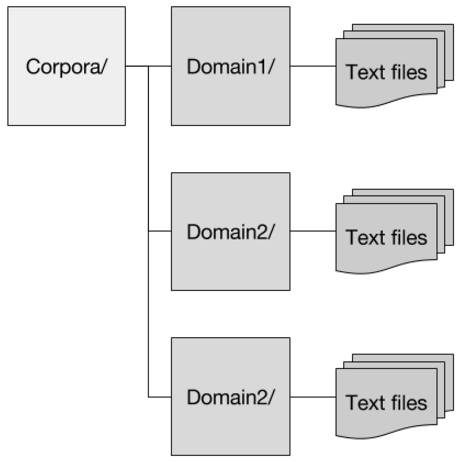
\includegraphics[width=.4\textwidth]{filestruct}
	\caption{Directory structure for the corpora.}
	\label{fig:Directorystructure}
\end{figure}

When accessing data from a corpus is required, the operation is as simple as looping over that directory and extracting the text from the text file. The code for doing that is shown in Figure  \ref{fig:Codeparse}.  Any additional corpus added to a domain directory will automatically be processed as additional data. The next important step for this project is to preprocess the raw text from the abstracts. As described in the previous section, text is divided into sub directories where files contain individual abstracts. 

\subsection{Preprocessing}

The first step in the preprocessing loads the text from a single corpora directory. For instance, choosing the directory ‘/computerscience’ will only load abstracts from the ‘Computer Science’ topic from which to preprocess text and eventually train our generator. Code is stripped of newline characters such that text will only be contiguous sentences.

\begin{figure}[!ht]
	\begin{verbatim}
	data = ""
	full_path = os.getcwd() + path
	for i in os.listdir(full_path):
	if i.endswith(".txt"):
	with open(full_path + '/' + i, 'r') 
	as f:
	data += f.read().replace('\n', ' ')
	\end{verbatim}
	
	\caption{Code to parse corpus.}
	\label{fig:Codeparse}
\end{figure}

Once the read is complete, the raw text is stripped of all text not contained in a whitelist. This whitelist contains all standard ASCII letters and digits, as well as a list of allowed characters. Manual inspection of the text proved the whitelist to be critical to guarantee no other special characters were included in the final data. Due to the need for sentence/word parsing as well as keeping hyphenated words or words with asterisks, certain popular in text characters such as periods ‘.’, spaces ‘ ‘, hyphens ‘-’, and asterisks ‘*’ are permitted and included in the whitelist. 

After the data is read in and compared against the whitelist, sentences are parsed. The parser moves over the text tokenizing every word and placing them into a list associated with a unique sentence. Decimal valued numbers are are found first with a regular expression, and are treated as individual tokens, otherwise, a string containing a period ‘.’ is considered the last word in the current sentence. The period is finally stripped from the sentence as clean tokenized words will be associated with our vocabulary. Future revisions may capture a variety of honorifics (e.g. ‘Dr.’) along associated with names of people as single tokens, however this is currently not supported.

The preprocessing of the raw data is now complete, however we must store this data in a way that we can utilize context free grammar (CFG). The preprocessing stage must store parts-of-speech tags of the clean sentences, parts-of-speech tags of the vocabulary, as well as N-Grams and their respective parts of speech. The format for storing this information is described in Figure 3.

\begin{figure}[!ht]
	\begin{verbatim}
	grammar_string = 
	""" 
	S -> NP VP
	PP -> P NP
	NP -> Det N | Det N PP | 'I'
	VP -> V NP | VP PP
	Det -> 'a' | 'my'
	N -> 'cow' | ‘pants’
	V -> 'through'
	P -> 'in'
	"""
	\end{verbatim}
	\caption{Code to parse corpus.}
	\label{fig:gramstring}
\end{figure}

The grammar string is formatted in two primary parts: the grammar rules, and vocabulary grouped by their respective parts of speech, separated by the pipe ‘|’ character. A grammar rule consists of an input part of speech tag, or the ‘S’ symbol denoting the start of a sentence, followed by a sequence of possible parts of speech tags that could follow that input. For the abstract generator, every new sentence in our corpus will generate a unique rule. In this way we guarantee the sentence will be grammatically correct while ensuring we have the minimum vocabulary to fill the rule. The final grammar string is used to create the NLTK grammar object for sentence generation. 
N-Grams are also collected during the preprocessing step. For the abstract generator, 2-Grams, 3-Grams, and 4-Grams are collected. These grams will be applied to post-generated text to improve their viability as readable and grammatically correct English sentences. A dictionary of N-Grams is created where the keys are  length of the gram (N), and the values are lists of tuples containing the N-Grams with their respective parts of speech.

\subsection{Sentence and Grammar Scoring}

After the creation of the grammar from the corpus, the grammar needs to have each elements scored to sort out what structures and words make sense and what structures and words don’t. There are a number of criteria which are used to score the grammar rules. Starting with a score of zero, some features add a negative score, and others a positive. A threshold is set, and grammar rules that fall below that threshold are not used in creating the context-free grammar (CFG). 
After the CFG is created, it can be used to generate new sentences from the rules. There are a huge number of potential sentences that can be generated from the CFG, so a way to select good sentences and bad sentences is a necessity. By evaluating and scoring the sentences, good sentences can be chosen from the generated sentences. Similar to how the grammar was scored, the sentences are scored against features to either add or subtract from their score. These features include number of unique words, as well as points for matching bi-grams, tri-grams, and quad-grams from the corpus. The highest scoring sentences are then selected for use in the abstract.

\subsection{Results and Summary}

Through a combination of techniques such as Context-Free Grammar and N-grams sentences can be generated. These sentences, if carefully selected, can be arranged intelligently to form more complete documents. By training a system on report abstracts, this system is able to use the content and structure of the abstracts to generate new abstracts. 


\addtolength{\textheight}{-12cm}   % This command serves to balance the column lengths
                                  % on the last page of the document manually. It shortens
                                  % the textheight of the last page by a suitable amount.
                                  % This command does not take effect until the next page
                                  % so it should come on the page before the last. Make
                                  % sure that you do not shorten the textheight too much.

%%%%%%%%%%%%%%%%%%%%%%%%%%%%%%%%%%%%%%%%%%%%%%%%%%%%%%%%%%%%%%%%%%%%%%%%%%%%%%%%



%%%%%%%%%%%%%%%%%%%%%%%%%%%%%%%%%%%%%%%%%%%%%%%%%%%%%%%%%%%%%%%%%%%%%%%%%%%%%%%%



%%%%%%%%%%%%%%%%%%%%%%%%%%%%%%%%%%%%%%%%%%%%%%%%%%%%%%%%%%%%%%%%%%%%%%%%%%%%%%%%




%%%%%%%%%%%%%%%%%%%%%%%%%%%%%%%%%%%%%%%%%%%%%%%%%%%%%%%%%%%%%%%%%%%%%%%%%%%%%%%%




%\begin{thebibliography}{99}

%\bibitem{c1} M. Romay, 'Hyperspectral Remote Sensing Scenes - GIC', Ehu.eus, 2015. [Online]. Available: http://www.ehu.eus/ccwintco/index.php?title=Hyperspectral_Remote_Sensing_Scenes. [Accessed: 26- Oct- 2015].



\bibliographystyle{plain}
% Single space the bibliography to save space.
%\begin{singlespace}
\bibliography{citations}
%\end{singlespace}




%\end{thebibliography}




\end{document}
